\documentclass[a4paper, 11pt]{article}
\usepackage[utf8]{inputenc} %interprete de simbolos en español
\usepackage[T1]{fontenc}
\usepackage[spanish]{babel}
\usepackage[margin=2.5cm, top=2.5cm, includefoot]{geometry}
\usepackage{url}
\usepackage{graphicx} % Insercción de imágenes
\usepackage{subfigure}
\usepackage[table,xcdraw]{xcolor} % detección de colores
\usepackage[most]{tcolorbox} % Insercción de cuadros en la portada
\usepackage{fancyhdr} % definir el estilo de la página
\usepackage[hidelinks]{hyperref} % gestión de hipervinculos
\usepackage{listings} % inserccón de codigo 
\usepackage{parskip} % arreglo de tabluación del documento
\usepackage[figurename=Figura]{caption} % cambiar nombre del caption de las fotos
\usepackage{smartdiagram} % insercción de diagramas
\usepackage{longtable} % Para tablas largas que ocupen varias páginas
\usepackage{zed-csp} % insercción de tablas
\usepackage[scaled]{helvet} % Fuente Helvetica
\usepackage[pages=some]{background} % imagen de fondo
\usepackage{sectsty} 
\usepackage{csquotes} % cargar para asegurar de que los textos citados se componen de acuerdos al idioma principal
\usepackage{tikz}
\usepackage{eso-pic}
\usepackage{stackengine} % opcion1 incluir para poner texto sobre imagen
\usepackage[backend=biber,style=apa,sorting=anyt]{biblatex} % uso de bibliografia
\addbibresource{referencias.bib} % referencia .bib

\renewcommand\familydefault{\sfdefault} % Quitar fuente default

\sectionfont{\fontsize{14}{16.8}\selectfont} % {Tamaño de fuente}{Salto de linea minimo 1.2}
\subsectionfont{\fontsize{12}{14.4}\selectfont}

% Declaración de variables
\newcommand{\logoTacticalOpsChile}{img/logo_tacticalops.png}
\newcommand{\logoTacticalOps}{img/to.png}

\newcommand{\nombreInforme}{Tactical Ops Chile}

% Imagen Head
\pagestyle{fancy}
\fancyhf{}
\rhead{\includegraphics[width=4cm]{\logoTacticalOps}}
\renewcommand{\headrulewidth}{0pt}

\begin{document}
\rfoot[]{\thepage} % número de página lado  derecho

    % Portada
    \begin{titlepage}
        \begin{center}
            {\Huge\ \textbf{\nombreInforme}}\par
            {\huge\ Reglamento Liga The Last Dance 2024}\par          
        \end{center}

        \vfill

        \begin{figure}[htb]
            \centering
            \includegraphics[scale=1.5]{\logoTacticalOpsChile}
        \end{figure} 
        
        \vfill

        \textbf{Equipo responsable: } Comunidad de Tactical Ops Chile\par\vspace{0.2cm}
        \textbf{Actualizado por: } BlackLung, Lalo, Slayer, Maiden\par\vspace{0.2cm}
        \textbf{Fecha: } 06-12-2024\par\vspace{0.3cm}

    \end{titlepage}
    \clearpage

    % -- Tabla de Contenido
    \tableofcontents
    \clearpage


    % Historial de cambios
    \section{Historial de cambios}
    
    \begin{longtable}{|p{2.5cm}|p{3.5cm}|p{6cm}|p{3cm}|}
        \hline
        \textbf{Fecha} & \textbf{Autor} & \textbf{Cambio realizado} & \textbf{Título} \\
        \hline
        \endfirsthead
        
        \hline
        \textbf{Fecha} & \textbf{Autor} & \textbf{Cambio realizado} & \textbf{Título} \\
        \hline
        \endhead
    
        \hline
        \multicolumn{4}{|r|}{Continúa en la siguiente página} \\
        \hline
        \endfoot
    
        \hline
        \endlastfoot
    
        18-12-2024 & Lalo, SlayeR, Maiden, BlackLung & Redacción de documento & Corrección inicial. \\ 
        \hline
        15-01-2025 & Representantes de cada clan & Se actualiza sección.  & Abandono de un clan. \\ 
        \hline
        10-02-2025 & Lalo y BlackLung & Se añadió una nueva sección grabación obligatoria y demos. & Nueva sección. \\ 
        \hline
        
    \end{longtable}
    \clearpage


    
    % -- Documento
     \section{Introducción}
     Bienvenidos a la Competición "The Last Dance" de Tactical Ops Chile. Este reglamento ha sido diseñado para garantizar una experiencia justa, competitiva y divertida para todos los participantes.

    El documento incluye las normas generales, las responsabilidades de los clanes, y los procedimientos necesarios para el desarrollo de los partidos. Nuestro objetivo es fomentar el juego limpio y fortalecer la comunidad de jugadores.

    Les invitamos a leer cuidadosamente cada sección del reglamento. Este será el marco de referencia que guiará cada aspecto de la competición, desde las inscripciones hasta las fases finales.

    ¡Les deseamos la mejor de las suertes a todos los clanes y jugadores en esta Liga!
    \clearpage

    \section{Inscripciones y Traspasos de Jugadores}
    
    \begin{itemize}
        \item Mínimo 7 jugadores y un máximo 11 por cada clan participante.
        \item Cada clan debe tener un representante oficial, quien será responsable de:
        \begin{itemize}
            \item Apoyar a la comunidad en lo necesario para el correcto desarrollo de la competición.
            Delegar sus funciones, si no puede cumplirlas, a una persona de confianza.
            \item El representante tiene la obligación de informar a su clan sobre las decisiones y acuerdos tomados en las reuniones convocadas por la comunidad.
        \end{itemize} 
                
        \item Cada jugador puede realizar un máximo de dos cambios de clan durante la competición, hasta la ronda número 7.
        \item Los equipos pueden realizar un máximo de tres cambios de jugadores a lo largo de la competición.
        \item Las inscripciones y cambios de clan deben notificarse en el grupo de WhatsApp de representantes con al menos 48 horas de anticipación antes del próximo partido.
        El representante debe editar su publicación original de inscripción para reflejar los cambios, indicando junto al nombre del jugador la hora y fecha del cambio. No se aceptarán publicaciones nuevas para este propósito.
      \end{itemize}
    \clearpage

    \section{Facultades y Obligaciones del Representante de Clan}
    
    \begin{itemize}
        \item Mantener informado a su equipo sobre los acuerdos y comunicados oficiales difundidos por los medios oficiales (como el grupo de WhatsApp de representantes).
        \item Durante un partido de liga, solo los representantes o sus delegados podrán gestionar la administración del encuentro. Esto debe acordarse entre los clanes al inicio del partido.
        \item El representante debe moderar o mirar al menos un partido por ronda de liga. Si no puede hacerlo, debe designar a un delegado.
    \end{itemize}

    \clearpage

    \section{Modalidad de Competición}

    \subsection{Etapa inicial}

    Los cinco mejores clanes de la tabla clasificarán directamente a la final presencial.
    En caso de empate, se resolverá siguiendo este orden de criterios:

    \begin{enumerate}
        \item  Resultados directos entre clanes empatados.
        \item  Diferencia de puntos entre ataque y defensa.
        \item  Total de puntos anotados.
        \item  Número de partidos ganados contra oponentes empatados (TB).
    \end{enumerate}
   
    Si el empate persiste, se realizará una definición en un único mapa, elegido por sorteo entre los mapas propuestos por los clanes.\par
    Ejemplo de tabla de clasificación:

    \begin{center}
        \begin{tabular}{||c c c c c c||} 
         \hline
         Nombre & Puntos & Partidos & Diferencia & Puntos Anotados & TB\\ [0.5ex] 
         \hline\hline
         Clan A & 39 & 13-0-1 & +60 & 85 & 2 \\ 
         \hline
         Clan B & 39 & 13-0-1 & +60 & 85 & 0 \\
         \hline
        \end{tabular}
    \end{center}

    Fecha 1: Clan A vs Clan B - Gana Clan A \par
    Fecha 8: Clan A vs Clan B - Gana Clan A

    \subsection{Etapa Final}

    La etapa final se disputará bajo un sistema de todos contra todos entre los cinco clanes clasificados. Cada clan se enfrentará entre sí, y los dos mejores equipos avanzarán a una final al mejor de tres mapas.

    \subsection{Clasificación y Pareos}
    La tabla de clasificación oficial será la definida y publicada en Challonge, la cual también servirá como referencia para los pareos.

    \subsection{Desempate en la Etapa Final}
    En caso de empate en la etapa final, se aplicará un sistema de overtime que consistirá en tres rondas por cada lado, con dos Endround por lado, hasta que se determine un ganador.

    \subsection{Selección de Mapas para la Final}

    Los líderes de los clanes propondrán mapas nuevos, La selección se realizará entre los representantes de los clanes.

    \subsection{Tiempo de Compra}

    \begin{itemize}
        \item Primer Preround: 20 segundos.
        \item Rondas siguientes: 10 segundos.
    \end{itemize}

    \clearpage

    \section{Reglas dentro del Juego}

    \subsection{Mínimo de Jugadores}
    Cada equipo deberá contar con un mínimo de 5 jugadores en el encuentro. Si no se alcanza este mínimo, el partido se declarará como WalkOver (WO).

    \subsection{Nicks Registrados}
    Todos los jugadores deben presentarse con su nick registrado, el cual debe ser claramente identificable.

    \subsection{WalkOver (WO)}
    Un partido declarado como WalkOver se adjudicará con una victoria para el equipo afectado, asignándole un puntaje equivalente al promedio de puntos de ataque de los demás clanes de su división (XX-0). Este puntaje se denominará Puntuación WalkOver (WO).

    \subsection{Tiempo de Espera}
    El tiempo máximo de espera para el inicio de un partido será de 15 minutos desde el horario pactado. (Propuesta sujeta a votación).

    \subsection{Administración del Match}
    Antes de iniciar el partido, se debe acordar quién será el encargado de administrar el encuentro. Dicho administrador deberá:

    \begin{itemize}
        \item Grabar una demo con el comando:
        \begin{lstlisting}
            forcedemorec all clanA_vs_clanB
        \end{lstlisting}
        \item Subir los resultados al canal de Discord designado para esta función. En caso de no ser posible, se habilitará un FTP para compartir los archivos.
        \item Actualizar resultados antes del inicio de la siguiente fecha.
    \end{itemize}

    \subsection{Grabación obligatoria y versiones permitidas}
    Antes de comenzar el partido, asegúrense de utilizar algunas de las versiones permitidas: v469d, v469e  RC7 release, Legacy v451. La versión v469RC4 release no está permitida.

Todos los jugadores deben grabar una demo y transmitir por Discord. Esto será verificado por cada capitán o representante designado para el partido. En caso de problemas relacionados con hardware o recursos de computador, se deja a criterio de ambos clanes decidir sobre esta práctica.

El observador designado para verificar la grabación debe tener el micrófono apagado y el modo de audífonos desactivado en Discord \ref{fig:discord}, en el canal donde esté observando. Esta designación debe realizarse antes del partido.

\begin{figure}[htb]
    \centering
    
\includegraphics[width=8cm]{img/discord.png}
    \caption{Reglas discord para observador.}
    \label{fig:discord}
\end{figure} 

    \subsection{Solicitud de Demos}
    Los representantes de los clanes pueden solicitar demos a los administradores dentro de un plazo máximo de dos rondas después del encuentro. Los jugadores deberán subir las demos al canal (DEMOS) de Discord en un plazo máximo de 48 horas tras la notificación. De no cumplir, los líderes de los clanes analizarán una posible sanción.

    \subsection{Uso del Chat “Say”}
    El chat “Say” está prohibido durante los partidos, excepto para los representantes de cada clan. Las infracciones serán sancionadas con un Warning. Si se reincide, el jugador recibirá un Mute durante el partido siguiente. El mute será levantado al finalizar el encuentro.

    \subsection{Uso de Bugs}
    Está estrictamente prohibido el uso de bugs o defectos de los mapas durante los partidos.

    \subsection{Reglas para Rehenes}

    \begin{itemize}
        \item Los rehenes pueden moverse durante todo el partido sin restricción de movimiento y sin que afecte el desarrollo del mapa.
        \item Si un rehén muere o se bugea, y hay tiempo para rescatarlo, el punto será para el “SF”. Si no hay tiempo, el punto será para los terroristas.
        \item La sanción será de un punto de partido si el rehén se Bugea intencionalmente.
    \end{itemize}

    
    \begin{figure}[htb]
        \centering
        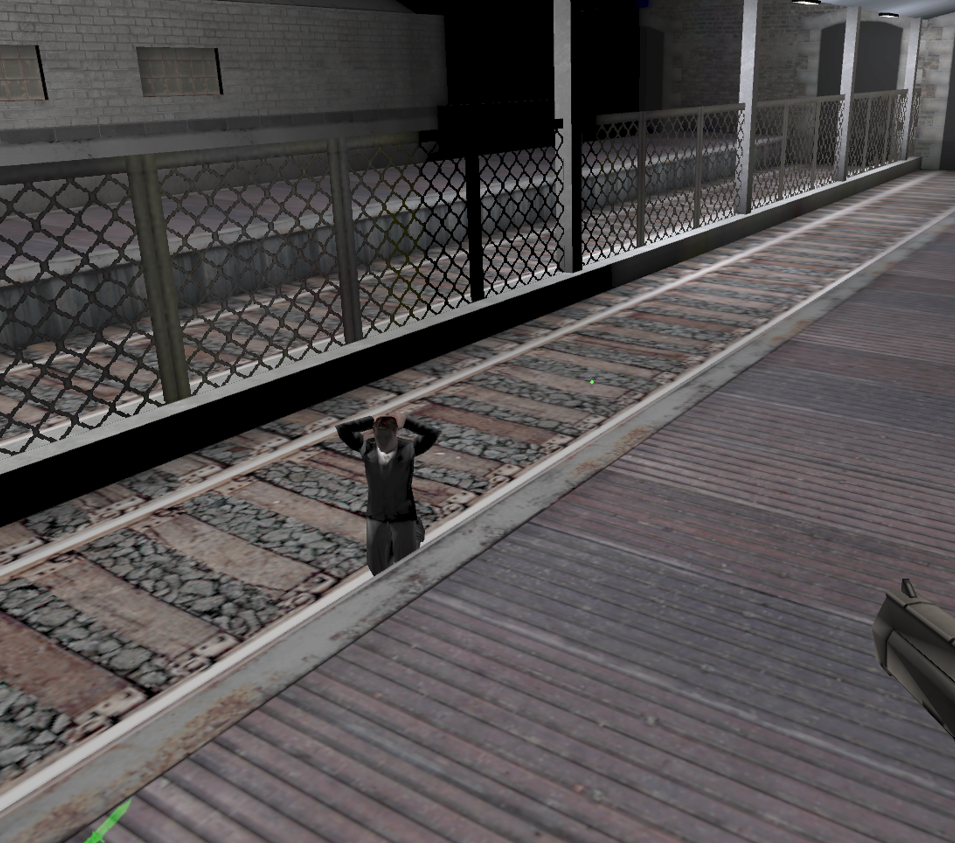
\includegraphics[width=8cm]{img/host_bug.png}
        \caption{Host no permitido.}
    \end{figure} 

    \subsection{Reglas para C4}

    Cuando un jugador provoca un bug intencionalmente, ya sea realizando TK (team kill) o desactivando de forma intermitente, no se considerará válido para el equipo "SF", incluso si se alega que fue causado por un BUG. 
    
    En cambio, si el bug ocurre debido a que el enemigo impide la desactivación y el jugador termina cayendo sobre la bomba, se evaluará el tiempo y las condiciones del round en cuestión (como el número de enemigos restantes, la disponibilidad de tiempo, entre otros factores). Si las circunstancias son favorables, se otorgará el punto correspondiente por BUG.

    En caso de cuestionamientos o simplemente no hay acuerdo entre los clanes, se solicitará el demo para aclarar las dudas, esto una vez terminado el partido.
    
    \begin{minipage}{0.40\textwidth}
        \centering
        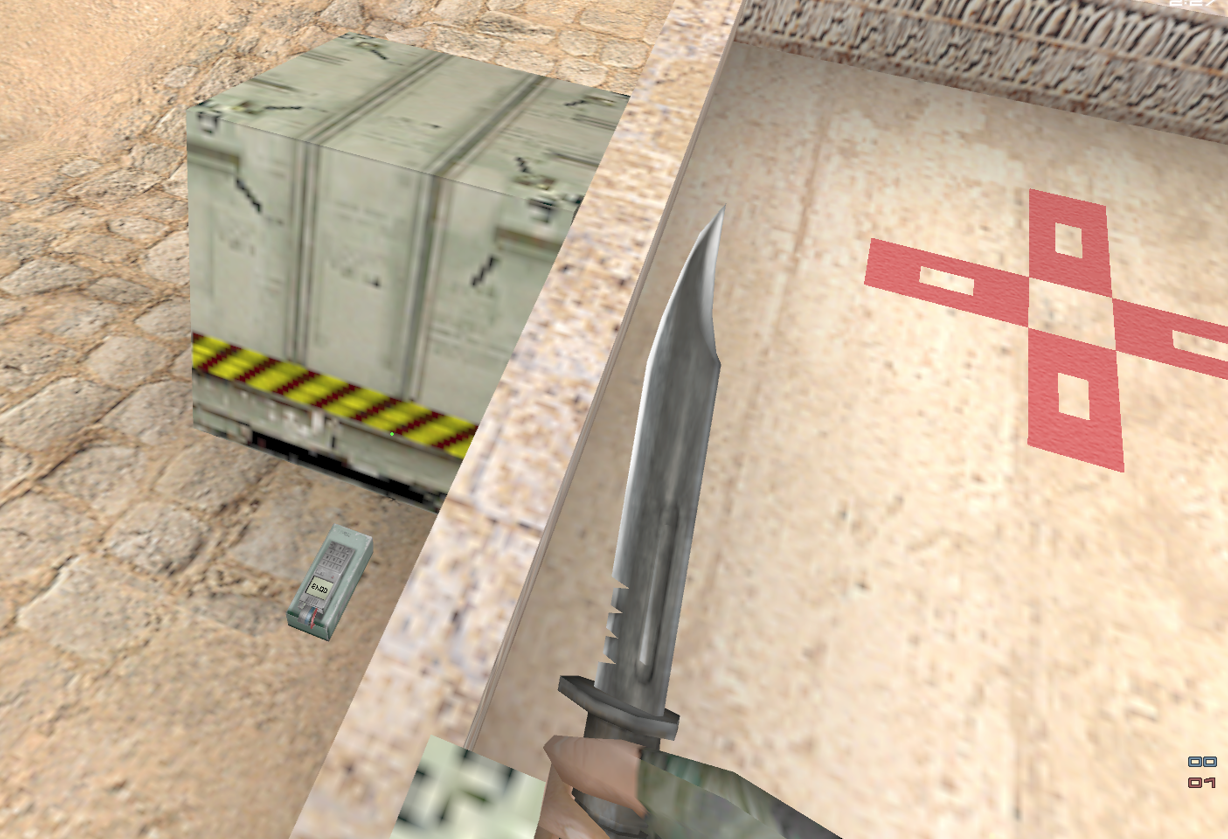
\includegraphics[width=\textwidth]{img/c4_bug.png}
        \captionof{figure}{C4 No permitida}
    \end{minipage}
    \hspace{0.05\textwidth}
    \begin{minipage}{0.45\textwidth}
        \centering
        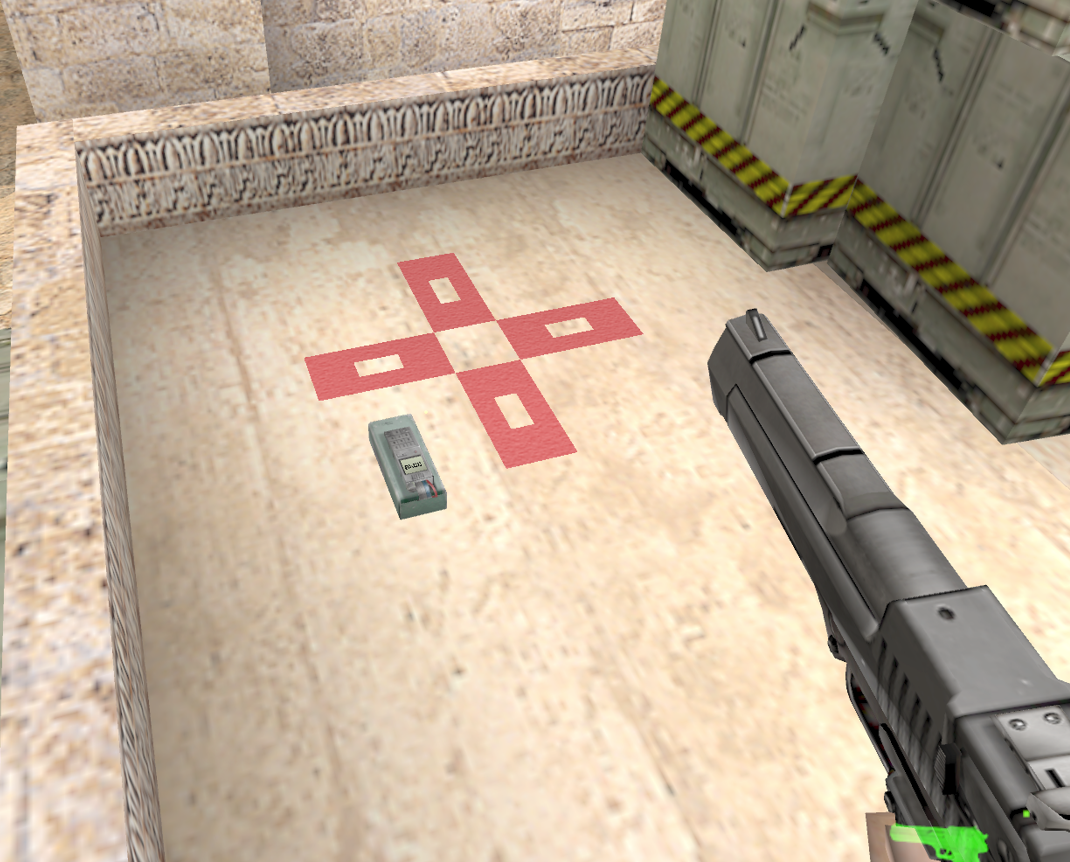
\includegraphics[width=\textwidth]{img/c4_nobug.png}
        \captionof{figure}{C4 permitida}
    \end{minipage}

    \subsection{Abandono de un Clan}
    Si un clan abandona la competición, será eliminado del Challonge, y los clanes que lo enfrentaban recibirán 0 puntos. tomando en cuenta que el clan nunca existió

    \subsection{Rondas por Partido}
    Cada partido consta de 24 rondas (12 por lado). Si un equipo abandona, los puntos faltantes serán otorgados al equipo que se mantenga con al menos 5 jugadores.

    \subsection{Comunicación Oficial}
    \begin{itemize}
        \item Solo se permite el uso del Discord oficial durante los partidos. Jugadores adicionales deben estar en mute.
        \item El Discord oficial es el siguiente \hyperlink{https://discord.gg/ajQxVbh8}{Totito}
    \end{itemize}

    \subsection{Cambios de Horario}
    Se permiten cambios de horario con 24 horas de antelación y con la aprobación del equipo contrario.

    \subsection{Fechas de Partidos}
    Los partidos deben jugarse entre domingo y miércoles. En caso de conflicto, el encuentro será obligatorio el domingo a las 23:00 horas.

    \subsection{Administración del Servidor}
    Solo se permite un administrador por equipo dentro del servidor.

    \subsection{Reclamos y Sugerencias}

    Todos los reclamos deben ser realizados por el representante del clan después del partido.

    \clearpage

    \section{Sanciones}
    Todas las sanciones están estipuladas en este reglamento en sus respectivos apartados. En caso de situaciones no contempladas o calificadas como "atípicas", se realizará una evaluación del caso en conjunto con los representantes de cada clan para determinar la sanción correspondiente.

    Ningún miembro del Staff ni de la administración podrá participar ni influir en las decisiones o sanciones que se apliquen si su clan está involucrado en el caso en cuestión.

    \subsection{Sobre el uso de trampas}
    Si un jugador es sorprendido utilizando trampas (Cheats) o modificando el archivo INI de manera no autorizada (por ejemplo, no lighting, no recoil u otras modificaciones), se procederá a imponer la sanción máxima de acuerdo con la resolución acordada entre los representantes de los clanes involucrados.

    Esta normativa aplica tanto para partidos de liga como para servidores de la comunidad. Cualquier modificación no autorizada será considerada como uso de trampas o manipulación indebida del archivo INI, lo que conllevará la sanción estipulada.


\end{document}